\documentclass[conference]{IEEEtran}
\usepackage{amsmath}
\usepackage{amsfonts}
\usepackage{amssymb}
\usepackage{amsthm}
\usepackage{lmodern}
\usepackage{array}
\usepackage{multirow}
\usepackage{amsmath,amssymb,amsthm}
\usepackage{subfigure}
\usepackage{lipsum}
\usepackage{fancyhdr}
\usepackage[T1]{fontenc}
\usepackage{times}
\DeclareMathAlphabet{\MATHIT}{OT1}{ptm}{m}{it}
\DeclareSymbolFont{Letters}{OML}{ztmcm}{m}{it}
\DeclareSymbolFontAlphabet{\mathNormal}{Letters}
\newcommand{\be}{\begin{equation}}
\newcommand{\ee}{\end{equation}}
\newcommand{\Bo}{\rule{2mm}{3mm}}
\usepackage[margin=1in,paperwidth=8.5in,paperheight=11in]{geometry}
\ifCLASSINFOpdf
\usepackage[pdftex]{graphicx}
\else
\usepackage[dvips]{graphicx}
\DeclareGraphicsExtensions{.eps}
\fi
\bibliographystyle{IEEEtran}
\def\ps@IEEEtitlepagestyle{
  \def\@oddfoot{\mycopyrightnotice}
  \def\@evenfoot{}
}
\def\mycopyrightnotice{
  {\footnotesize 978-1-4673-9802-2/16/\$31.00\textcopyright 2016 IEEE}
  \gdef\mycopyrightnotice{}
}
\fancyhead{}
\fancyfoot{}
\fancypagestyle{plain}{
        \fancyhead{}
        \fancyhead[C]{2016 Fifth International Conference On Recent Trends In Information Technology}
        \fancyfoot{}
        \fancyfoot[L]{978-1-4673-9802-2/16/\$31.00 {\copyright}2016 IEEE}
}
\pagestyle{fancy}
\hyphenation{op-tical net-works semi-conduc-tor}


\begin{document}
  \thispagestyle{fancy}
  \def\ieeenotice{978-1-4673-9802-2/16/\$31.00 {\copyright}2016 IEEE}
  \def\confinfo{2016 Fifth International Conference On Recent Trends In Information Technology}
   \chead{\confinfo}
  \renewcommand{\headrulewidth}{0pt}

\renewcommand{\headrulewidth}{0pt}
\title{Dynamics of Attack of Malicious Codes on the Targeted Network: Effect of Firewall}

\author{Ashish Bhargava, Durgesh Kumar Soni, Palash Jain, Joydip Dhar \\ ABV-Indian Institute of Information Technology and Management, \\
Gwalior-474015, Madhya Pradesh  \\}

\maketitle
\thispagestyle{fancy}
\begin{abstract}
In this work, a mathematical model has been developed to analyze the spread of a distributed attack on critically targeted resources in a network using firewall security coefficient. The model provides an epidemic framework with two sub-frameworks to consider the difference between the overall behavior of the attacking population and the targeted population. The targeted population and attacking population  is divided into five compartments of nodes, viz. Susceptible-Latent-Breaking out-Recovered-Antidotal. With cyber mass action incidence, the boundedness of the system, the feasibility of equilibrium states and their stabilities are analyzed. Basic reproduction number ${{\cal R}}_{0}$ is calculated and it is observed that when ${{\cal R}}_{0}<1$, then the system will have malicious code free stable steady state. Again, when ${{\cal R}}_{0}>1$, then endemic steady state exists and will be locally asymptotically stable. The impact of firewall security rule base in controlling transmission of malicious objects is analyzed. We are taking firewall security as a media coverage factor in our computer network model of malicious code propagation. Asymptotic local stability method is used as an alternate to find the stability of the system. Finally, a sensitivity analysis of the system parameters for basic reproduction number and endemic equilibrium points has been carried out using normalized forward sensitivity index. Numerical experimentation has been carried out to simulate the system of equations in support of analytical findings.
\end{abstract}

\section{Introduction}
Malicious code does not just affect one computer, it can also get into the networks and spread. It can send messages through email and steal information or cause even more damage by deleting files. It is a computer program that operates on behalf of a potential intruder to aid in attacking a system or network. Malicious code can come in various other forms. A common type of malicious code is the virus, which is a little program attaching to other programs or files and will copy itself in a computer and even spread to other networked computers. Viruses can range from being relatively harmless to causing significant damage to a system.
\indent Worms are pieces of malicious code making copies of itself. Conditions have to be right for a worm to proliferate. They are created mainly using scripting languages.

Trojan horses are forms of malicious code appearing as safe software. But that is how they get into a computer. They may be hiding inside another program and be installed with an otherwise safe program. Sometimes they give someone in a remote location control of the victim's computer \cite{goswami2012information}.

These agents acts as a serious threat to the security of the computer networks. An infected computer can have significance performance degradation when attacked by the malicious codes in breaking-out state. Malicious codes have a potential of replicating themselves from one computer to another without you being aware that your machine has become infected \cite{wang2015worm}. In the era of cloud computing, this threat has become more and more serious as new variants of existing viruses including some new ones are continuously emerging and increasing the vulnerability of the system. This calls for a need to continuously develop new counter-defense mechanisms. The evolution trend of viruses cannot be predicted and thus universal proposal for their avoidance and control cannot be recommended \cite{yang2012towards}.

In a certain sense, malicious codes spread in computer network is epidemic in nature, i.e., the propagation of computer viruses in a system of interacting and integrated computers could be compared with disease transmission in biological world \cite{brady2015editor}. Keeping the epidemic nature of virus spread certain mathematical models are developed. With the continuous emergence of new type of attacks, there is a need to improve the propagation models. Mathematical modeling has become an important tool in analyzing the spread and control of malicious codes in computer networks. Mathematical models take into account the main factors that govern spread of virus, such as transmission and recovery rates, and predict how the viruses will spread over a period of time.
Only a small fraction of all known viruses have appeared in real incidents, partly because many viruses are below the theoretical epidemic threshold. The observed sub-exponential rate of viral spread can be explained by models of localized software exchange. A surprisingly small fraction of machines in well-protected business environments are infected. This may be explained by a model in which, once a machine is found to be infected, neighboring machines are checked for viruses. This "kill signal" idea could be implemented in networks to greatly reduce the threat of viral spread.
\thispagestyle{plain}
\newpage
\section{Model Development}
We consider two groups of computer nodes, namely, targeted nodes and attacker nodes. In this model attacker-targeted population is divided into five compartments namely Susceptible, Latent, Breaking-out, Antidotal and Recovered compartment. Here we have divided total computer nodes $T$ into ten classes, namely, $S(t)$ of non- infected targeted computers subjected to possible infection; $S_1(t)$ of non-infected computers of attacker class; $A(t)$, $A_1(t)$ non-infected computers of targeted and attacker class equipped with fully effective antivirus program; $L(t)$, $L_1(t)$ infected computers of targeted and attacker class with virus in latent state; $B(t)$, $B_1(t)$ infected computers of targeted and attacker class with virus in breaking-out state and recovered class population $R(t)$, $R_1(t)$ of recovered ones from the infection in targeted and attacker class respectively. The Schematic diagram of the model shown in the figure\ref{sf1}. Here it is assumed that the population has a homogeneous spatial distribution and the mixing of hosts follow the law of mass action, i.e., the local population density is a constant through the total population size \cite {piqueira2005epidemiological,piqueira2008dynamic,mishra2007seirs,mishra2010seiqrs}. Targeted population $N(t)=S(t)+L(t)+B(t)+R(t)+A(t)$   and attacker population $N_1(t)=S_1(t)+L_1(t)+B_1(t)+R_1(t)+A_1(t)$.

\indent The primary goal of this model is to theoretically study the impact of firewall security rule base in controlling transmission of malicious objects \cite{misra2014capturing}. Many researchers investigated the impact of media awareness in biological disease spread using mathematical modeling used transmission coefficient function of the form $\beta(I)=\beta e^{-mI}$ and established that multiple positive equilibria are possible when the media effect is sufficiently strong \cite{cui2008impact, liu2008impact, sahu2012, sahu2015dynamics}. Similarly we are taking firewall security as a media coverage factor in our computer network model of malicious code propagation. Non-linear function of the form $\beta(I) = c_1 - c_2 f (I),$ is incorporated in the transmission term to investigate the effect of firewall security, where $f(I)=\frac{I}{m+I}$. In the modeling of malicious code propagation, the incidence function plays a very important role. In many models, the bilinear incidence rate $\beta \tilde{S}\tilde{I}$ and the standard incidence rate $\frac{\beta\tilde{S}\tilde{I}}{N}$ are frequently used, where $\beta$ measures the effect of both the propagation of the malicious code and the contact transmission rates. However, these incidence functions do not consider the impact of firewall security to the spread and control of malicious code propagation \cite{sun2014impact}.

\indent The use of firewall security and alert has been found beneficial for reducing malicious code propagation. Initially researchers used media induced transmission rate of the form $\beta(I)=\beta e^{-mI}$ which has two major limitations. We consider firewall induced transmission rate as $\beta(I)=\beta e^{-m\frac{I}{N}}$ in the proposed model which is more reasonable than $\beta(I)=\beta e^{-mI},$ because $\beta e^{-mI}\rightarrow 0$ as $I\rightarrow \infty$, independent of the value of $m$. Since the firewall security and alertness are not the intrinsic deterministic factor responsible for the transmission, hence it is reasonable to assume that the transmission rate cannot be reduced below a certain level merely through firewall security alert. Moreover, even for a fixed m, the minimum transmission rate differs for different population sizes, which is not very realistic. On the other hand, $min\{\beta e^{-m\frac{I}{N}}\} = \beta e^{-m}$ that remains unchanged with respect to the total population size.\\


\begin{figure}[h]
 %\begin{minipage}{0.5\columnwidth}
  \centering
  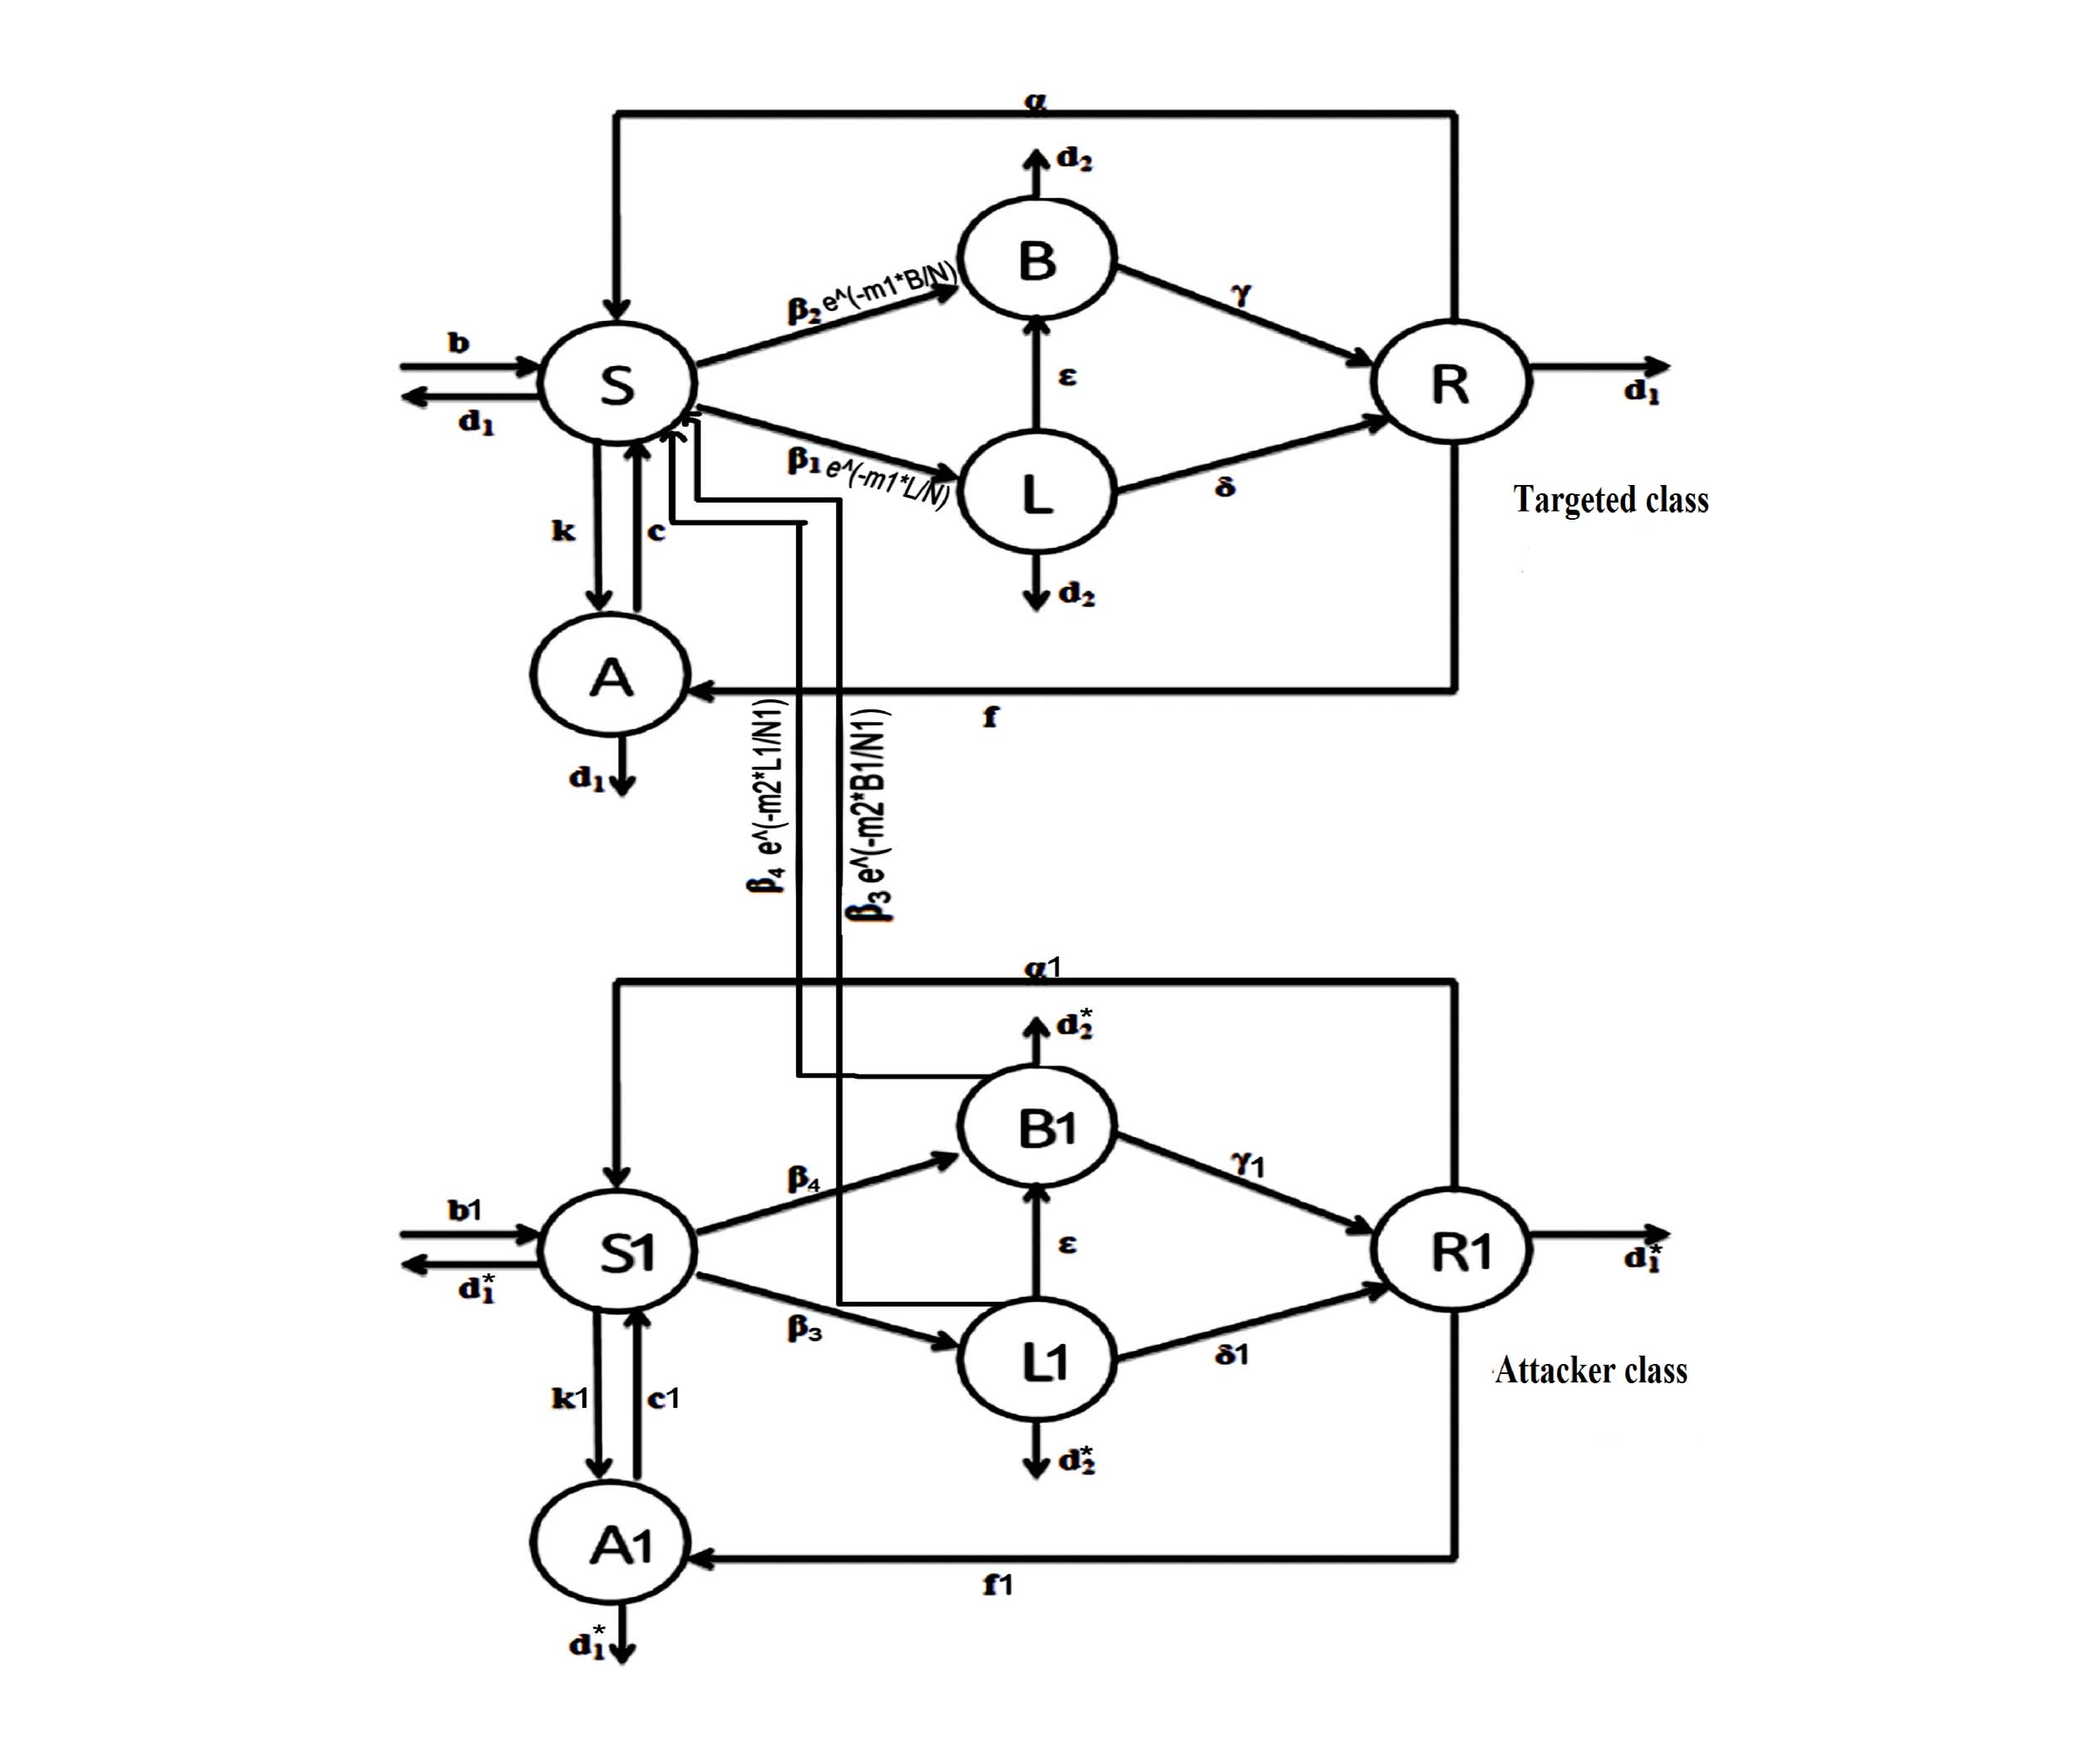
\includegraphics[width=1.3\columnwidth, clip=true]{modelcopy1.eps}
  \caption{Schematic Flow of Proposed Model}\label{sf1}
  %\end{minipage}
 \end{figure}


\normalfont

\section{Proposed Mathematical Model}
Keeping in view the transmission rates of the schematic flow diagram which is shown in the figure \ref{sf1}. The system is governed by following set of ordinary differential equations and its parameters are discussed in table \ref{newtab}:\\

\textbf{For Targeted nodes:}\\
\begingroup
\everymath{\scriptstyle}
\scriptsize
\begin{eqnarray}
\frac{d\tilde{S}}{d\tilde{t}} &=& b-\tilde{\beta_2} e^{-m_1 \frac{\tilde{B}}{\tilde{N}}}\tilde{S} \frac{\tilde{B}}{\tilde{N}}-\tilde{\beta_1} e^{-m_1\frac{\tilde{L}}{\tilde{N}}} \tilde{S}\frac{\tilde{L}}{\tilde{N}}-\tilde{k}\tilde{S}\tilde{A}+\tilde{c}\tilde{A}-\tilde{d_1}\tilde{S} + \nonumber \\
&& \tilde{\alpha} \tilde{R}-\tilde{\beta_2} e^{-m_2 \frac{\tilde{B_1}}{\tilde{N_1}}} \tilde{S} \frac{\tilde{B_1}}{\tilde{N_1}} -\tilde{\beta_1} e^{-m_2 \frac{\tilde{L_1}}{\tilde{N_1}}} \tilde{S} \frac{\tilde{L_1}}{\tilde{N_1}},
\label{se1}
\end{eqnarray}
\endgroup
\begingroup
\everymath{\scriptstyle}
\scriptsize
\be
\frac{d\tilde{B}}{d\tilde{t}}=\tilde{\beta_2} e^{-m_1 \frac{\tilde{B}}{\tilde{N}}} \tilde{S}\frac{\tilde{B}}{\tilde{N}}-\tilde{d_2}\tilde{B}+\tilde{\epsilon} \tilde{L}-\tilde{\gamma} \tilde{B}+\tilde{\beta_2} e^{-m_2\frac{\tilde{B_1}}{\tilde{N_1}}}\tilde{S}
\frac{\tilde{B_1}}{\tilde{N_1}},
\label{se2}
\ee
\endgroup
\begingroup
\everymath{\scriptstyle}
\scriptsize
\be
\frac{d\tilde{L}}{d\tilde{t}}=\tilde{\beta_1} e^{-m_1\frac{\tilde{L}}{\tilde{N}}} \tilde{S}\frac{\tilde{L}}{\tilde{N}}-\tilde{d_2}\tilde{L}-\tilde{\epsilon}\tilde{L}-
\tilde{\delta} \tilde{L}+ \tilde{\beta_1} e^{-m_2\frac{\tilde{L_1}}{\tilde{N_1}}}\tilde{S}\frac{\tilde{L_1}}{\tilde{N_1}},
\label{se3}
\ee
\endgroup
\begingroup
\everymath{\scriptstyle}
\scriptsize
\be
\frac{d\tilde{R}}{d\tilde{t}}=\tilde{\gamma} \tilde{B}+\tilde{\delta}\tilde{L}-\tilde{f}\tilde{R}-\tilde{\alpha} \tilde{R}-\tilde{d_1}\tilde{R},
\label{se4}
\ee
\endgroup
\begingroup
\everymath{\scriptstyle}
\scriptsize
\be
\frac{d\tilde{A}}{d\tilde{t}}=\tilde{f}\tilde{R}-\tilde{d_1}\tilde{A}+ \tilde{k} \tilde{S}\tilde{A}-\tilde{c}\tilde{A},
\label{se5}
\ee
\endgroup

\textbf{For Attacker nodes:}\\
\begingroup
\everymath{\scriptstyle}
\scriptsize
\begin{eqnarray}
\frac{d\tilde{S_1}}{d\tilde{t}} &=& b_1-\tilde{\beta_4}\tilde{S_1}\tilde{B_1} -\tilde{\beta_3} \tilde{S_1}\tilde{L_1}-\tilde{k_1} \tilde{S_1}\tilde{A_1}+\tilde{c_1}\tilde{A_1} \nonumber\\
&-& \tilde{d_3}S_1+\tilde{\alpha_1}\tilde{R_1},
\end{eqnarray}
\endgroup
\begingroup
\everymath{\scriptstyle}
\scriptsize
\begin{eqnarray}
\frac{d\tilde{B_1}}{d\tilde{t}} &=& \tilde{\beta_4}\tilde{S_1}\tilde{B_1}-\tilde{d_4}\tilde{B_1}+\tilde{\epsilon_1}L_1-\tilde{\gamma_1}{B_1},
\end{eqnarray}
\endgroup
\begingroup
\everymath{\scriptstyle}
\scriptsize
\begingroup
\everymath{\scriptstyle}
\scriptsize
\begin{eqnarray}
\frac{d\tilde{L_1}}{d\tilde{t}} &=& \tilde{\beta_3}\tilde{S_1}\tilde{L_1}-\tilde{d_4}\tilde{L_1}-\tilde{\epsilon_1}L_1-\tilde{\delta_1}{L_1},
\end{eqnarray}
\endgroup
\begingroup
\everymath{\scriptstyle}
\scriptsize
\begin{eqnarray}
\frac{d\tilde{R_1}}{d\tilde{t}} &=& \tilde{\gamma_1} \tilde{B_1} + \tilde{\delta_1}\tilde{L_1}-\tilde{f_1}\tilde{R_1}-\tilde{\alpha_1} \tilde{R_1}-\tilde{d_3}\tilde{R_1},
\end{eqnarray}
\endgroup
\begingroup
\everymath{\scriptstyle}
\scriptsize
\begin{eqnarray}
\frac{d\tilde{A_1}}{d\tilde{t}} &=& \tilde{f_1}\tilde{R_1}-\tilde{d_3}\tilde{A_1}+\tilde{k_1}\tilde{S_1}\tilde{A_1}-\tilde{c_1}\tilde{A_1}.
\end{eqnarray}
\endgroup

\normalsize
\noindent
where, all the system parameters are positive and described in table \ref{newtab}.
\begin{center}
\begin{table}[ht!]
\caption{Parameters Description}\label{newtab}
%\scriptsize
%\footnotesize
\begin{tabular}{|c|l|}
  \hline
  % after \\: \hline or \cline{col1-col2} \cline{col3-col4} ...
  \textbf{Parameters} & \textbf{Description }\\
  \hline
  $b,b_1$ & Recruitment rates\\
  \hline
  $d_1,d_2$ & Natural death rate of attacker and \\
  & targeted population nodes\\
  \hline
  $\beta,\beta_1$ & Contact rate from susceptible class to \\
  & latent class;(in the absence of firewall) \\
  \hline
  $\gamma,\gamma_1$ & Rate of recovery of computers with \\
  & malicious codes in breaking-out state \\
  \hline
  $\delta,\delta_1$ & Rate of recovery of computers with \\
  & malicious codes in latent state \\
  \hline
  $d_3,d_4$ & Death rate in infected class(death \\
  & due to infection and natural death) \\
  \hline
  $\epsilon,\epsilon_1$& Conversion rate of malicious codes \\
  & from latent to braking-out state\\
  \hline
  $f,f_1$ & Conversion rate of recovered nodes\\
  & into antidotal nodes \\
  \hline
  $c,c_1$ & Conversion rate of antidotal nodes \\
  & into susceptible nodes \\
  \hline
  $k,k_1$ & Conversion rate of susceptible nodes \\
  & into antidotal nodes \\
  \hline
  $\alpha,\alpha_1$ & Conversion rate of recovered nodes \\
  & into susceptible nodes \\
  \hline
  $m_1, \ m_2$ & Firewall security coefficients\\
  \hline
\end{tabular}
\end{table}
\end{center}

\noindent Non-dimensionalise the above system using,\\
\noindent
$S=\frac{\tilde{S}}{\tilde{N}}$, $B=\frac{\tilde{B}}{\tilde{N}}$, $L=\frac{\tilde{L}}{\tilde{N}}$, $R=\frac{\tilde{R}}{\tilde{N}}$,
$A=\frac{\tilde{A}}{\tilde{N}}$, $S_1=\frac{\tilde{S_1}}{\tilde{N_1}}$, $B_1=\frac{\tilde{B_1}}{\tilde{N_1}}$, $L_1=\frac{\tilde{L_1}}{\tilde{N_1}}$,
$R_1=\frac{\tilde{R_1}}{\tilde{N_1}}$, $A_1=\frac{\tilde{A_1}}{\tilde{N_1}}$, $t=\tilde{d_1}\tilde{t}$, $N=\frac{\tilde{N}}{\tilde{N^0}}$,
$N_1=\frac{\tilde{N_1}}{\tilde{{N_1}^0}}$.
Where, $\tilde{N^0}=\frac{b}{\tilde{d_1}}$ and $\tilde{{N_1}^0}=\frac{b}{\tilde{d_3}}$. Targeted population and attacker population parameters $\tilde{d_1}$ and $\tilde{d_3}$ respectively become $\beta_1=\frac{\tilde{\beta_1}}{\tilde{d_1}}$, $\beta_3=\frac{\tilde{\beta_3}}{\tilde{d_3}}$.


%The equivalent non-dimensional system is given by:\\
%
%\textbf{Targeted population:}\\
%\begingroup
%\everymath{\scriptstyle}
%\scriptsize
%\begin{eqnarray}
%\frac{dS}{dt} &=& \frac{(1-S)}{N}-\beta_2 e^{-m_1B} SB-\beta_1 e^{-m_1L} SL-kSAN + \nonumber\\
%&& cA  - S + \alpha R  -\beta_2 e^{-m_2B_1} SB_1-\beta_1 e^{-m_2L_1} SL_1 + \nonumber\\
%&& S^2+d_2SL+d_2SB+RS+AS,
%\end{eqnarray}
%\endgroup
%\begingroup
%\everymath{\scriptstyle}
%\scriptsize
%\begin{eqnarray}
%\frac{dB}{dt} &=& \beta_2 e^{-m_1B} SB-d_2B+\epsilon L-\gamma B+\beta_2 e^{-m_2B_1} SB_1 - \nonumber\\
%&& \frac{B}{N}+BS+d_2B^2+d_2BL+BR+BA,
%\end{eqnarray}
%\endgroup
%\begingroup
%\everymath{\scriptstyle}
%\scriptsize
%\begin{eqnarray}
%\frac{dL}{dt} &=& \beta_1 e^{-m_1L} SL-d_2L-\epsilon L-\delta L+\beta_1 e^{-m_2L_1} SL_1 -  \nonumber\\
%&& \frac{L}{N}+SL + d_2L^2 + d_2BL+RL+AL,
%\end{eqnarray}
%\endgroup
%\begingroup
%\everymath{\scriptstyle}
%\scriptsize
%\begin{eqnarray}
%\frac{dR}{dt} &=& \gamma B+\delta L-fR-\alpha R-R-\frac{R}{N}+RS+d_2RB + \nonumber\\
%&& d_2RL+R^2+RA,
%\end{eqnarray}
%\endgroup
%\begingroup
%\everymath{\scriptstyle}
%\scriptsize
%\begin{eqnarray}
%\frac{dA}{dt} &=& fR-A-cA+kASN-\frac{A}{N}+AS+d_2AB + \nonumber\\
%&& d_2AL+AR+A^2,
%\end{eqnarray}
%\endgroup
%
%\textbf{Attacker population:}\\
%\begingroup
%\everymath{\scriptstyle}
%\scriptsize
%\begin{eqnarray}
%\frac{dS_1}{dt} &=& \frac{(1-S_1)}{N_1}-\beta_4 S_1 B_1 N_1-\beta_3 S_1 L_1 N_1-k_1 S_1A_1N_1 + \nonumber\\
%&& c_1A_1-S_1+\alpha_1 R_1+S_1^2+d_3S_1B_1 + \nonumber\\
%&& d_3S_1L_1+S_1R_1+S_1A_1,
%\end{eqnarray}
%\endgroup
%\begingroup
%\everymath{\scriptstyle}
%\scriptsize
%\begin{eqnarray}
%\frac{dB_1}{dt} &=& \beta_4S_1B_1N_1-d_3B_1+\epsilon_1L_1-\gamma_1B_1-\frac{B_1}{N_1}+B_1S_1 + \nonumber\\
%&& d_3{B_1}^2+d_3B_1L_1
%+B_1R_1+B_1A_1,
%\end{eqnarray}
%\endgroup
%\begingroup
%\everymath{\scriptstyle}
%\scriptsize
%\begin{eqnarray}
%\frac{dL_1}{dt} &=& \beta_3S_1L_1N_1-d_3L_1-\epsilon_1L_1-\delta_1L_1-\frac{L_1}{N_1}+S_1L_1 + \nonumber\\
%&& d_3{L_1}^2+d_3B_1L_1+R_1L_1+A_1L_1,
%\end{eqnarray}
%\endgroup
%\begingroup
%\everymath{\scriptstyle}
%\scriptsize
%\begin{eqnarray}
%\frac{dR_1}{dt} &=& \gamma_1B_1+\delta_1L_1-f_1R_1-\alpha_1R_1-R_1-\frac{R_1}{N_1}+R_1S_1 + \nonumber\\
%&& d_3R_1B_1+d_3R_1L_1+{R_1}^2+R_1A_1,
%\end{eqnarray}
%\endgroup
%\begingroup
%\everymath{\scriptstyle}
%\scriptsize
%\begin{eqnarray}
%\frac{dA_1}{dt} &=& f_1R_1-A_1-c_1A_1+k_1A_1S_1N_1-\frac{A_1}{N_1}+A_1S_1 + \nonumber\\
%&& d_3A_1B_1+d_3A_1L_1+A_1R_1+{A_1}^2,
%\end{eqnarray}
%\endgroup
%

\section{Results and Discussion}
In this section we will discuss various analyses and results obtained :

\subsection{Boundedness of the System}
Our targeted system is bounded, in the simply connected compact set
\footnotesize \[
\Omega_\kappa =  \left\{(S,L,B,R,A) \in R^5_+ : S+L+B+R+A \leq \frac{b}{\tilde{d}} + \kappa \right\}\]
\normalsize
is positively invariant for the SLBRAS model. Similarly boundedness follows for attacking population.

\subsection{Basic Reproduction Number}
The basic reproduction number $R_{0}$, is defined as the expected number of secondary cases produced by a single infection in a completely susceptible population. It is considered as one of the most useful threshold parameters to characterize the malicious object propagation. It can be obtained by taking the derivative of infection classes, i.e., $2^{nd}$ and $3^{rd}$ equations of attacker system and $2^{nd}$ and $3^{rd}$ equations of targeted system.\\
Let $x$= $(L, B, L_{1}, B_{1})$ then,

\indent $\frac{dx}{dt} = \cal{F}-\cal{V},$

\noindent where $S$, $S_1$ is the node density of susceptible class and $A$, $A_1$ is the node density of antidotal class of targeted and attacker population respectively in malicious codes - free equilibrium state. In this model we have four such states $E_1$, $E_2$, $E_3$ and $E_4$ and hence we have four basic reproduction number $R_{01}$, $R_{02}$, $R_{03}$ and $R_{04}$ respectively.
Value of $R_{01}$, $R_{02}$, $R_{03}$ and $R_{04}$ are:

\noindent For equilibrium state $E_1:$ $S=1$, $A=0$, $S_1=1$, $A_1=0$ and hence,

$R_{01}$=$max$\{$\frac{1+{\beta}_1}{1+d_2+\delta+\varepsilon}$,$\frac{1+{\beta}_3}{1+d_3+{\delta}_1+{\varepsilon}_1}$,$\frac{1+{\beta}_2}{1+d_2+\gamma}$,
$\frac{1+{\beta}_4}{1+d_3+{\gamma}_1}$\}.

\subsection{Local Asymptotic Stability}
Now, we explore the local stability of malicious codes-free and endemic equilibrium. Equilibrium state $E_1$ will be locally asymptotically stable when all  eigenvalues of $J_ {01}$ variational matrix are negative or having negative real parts.
Clearly, if ${{\cal R}}_{01}<1$, then all the eigenvalues will have negative real parts. Hence, the malicious code free equilibrium $E_1$ is locally asymptotically stable, if ${\cal R}_{01} < 1$ and unstable, if ${\cal R}_{01} > 1$.

The basic reproduction number can be obtained by taking the derivative of infection classes, i.e., $2^{nd}$ and $3^{rd}$ equations of attacker system and $2^{nd}$ and $3^{rd}$ equations of targeted system. Let $x$= $(L, B, L_{1}, B_{1})$ then,

$\frac{dx}{dt} = \cal{F}-\cal{V},$

\noindent where,
\begingroup
\everymath{\scriptstyle}
\scriptsize
$\cal{F}$ =
    ${\left(
    \begin{array}{c}
      {\beta}_2 e^{-m_1 B} S B+{\beta}_2 e^{-m_2 B_1} S B_1+B S \\
      {\beta}_1 e^{-m_1 L} S L+{\beta}_1 e^{-m_2 L_1} S L_1+L S  \\
      {\beta}_4 S_1 N_1 B_1+B_1 S_1 \\
      {\beta}_3 S_1 N_1 L_1+S_1 L_1 \\
    \end{array}
  \right) },$
\endgroup

\begingroup
\everymath{\scriptstyle}
\scriptsize
 $\cal{V}$ =
 ${\left(
   \begin{array}{c}
     d_2 B -\varepsilon L +\gamma B +\frac{B}{N} -d_2 B^2 -B R - B A - d_2 B L \\
     d_2 L +\varepsilon L +\delta B +\frac{L}{N} -d_2 L^2 - R L - A L - d_2 B L \\
     d_3 B_1 - \varepsilon L_1+\gamma B_1 +\frac{B_1}{N_1}-d_3 L_1 B_1 -d_3 {B_1}^2 -B_1 R_1 -B_1 A_1 \\
     d_3 L_1 + \varepsilon L_1+\delta L_1 +\frac{L_1}{N_1}-d_3 L_1 B_1 -d_3 {L_1}^2 -L_1 R_1 -L_1 A_1 \\
   \end{array}
 \right)},$
\endgroup \\

\noindent we get, F(Jacobian of $\cal{F}$  at malicious codes-free equilibrium)= \\
\begingroup
\everymath{\scriptstyle}
\scriptsize
     $\left(
       \begin{array}{cccc}
         ({\beta}_2+1) S & 0 & {\beta}_2 S & 0 \\
         0 & ({\beta}_1+1) S & 0 & {\beta}_1 S \\
         0 & 0 & ({\beta}_4+1) S_1 & 0 \\
         0 & 0 & 0 & ({\beta}_3+1) S_1 \\
       \end{array}
     \right),$
\endgroup \\

\noindent and, V(Jacobian of $\cal{V}$  at malicious codes-free equilibrium)= \\
\begingroup
\everymath{\scriptstyle}
\scriptsize
 $\left(
   \begin{array}{cccc}
     \gamma-A+d_2+1 & -\varepsilon & 0 & 0 \\
     0 & \varepsilon-A+\delta+d_2+1 & 0 & 0 \\
     0 & 0 & {\gamma}_1-A_1+d_3+1 & -{\varepsilon}_1 \\
     0 & 0 & 0 & d_3-A_1+{\varepsilon}_1+{\delta}_1+1 \\
   \end{array}
 \right).$
\endgroup \\
\\

where, F is the matrix of rates of secondary infection and V is the matrix of rates of transmission. Then, the basic reproductive number $R_0$ is defined as the dominant eigenvalue of $FV^{-1}$. \\
\begingroup
\everymath{\scriptstyle}
\scriptsize
$R_0 = max\left\{\frac{S(1+{\beta}_1)}{1+d_2+\delta+\varepsilon-A},\frac{S_1(1+{\beta}_3)}{1+d_3+{\delta}_1+{\varepsilon}_1-A_1},
\frac{S(1+{\beta}_2)}{1+d_2+\gamma-A},\frac{S_1(1+{\beta}_4)}{1+d_3+{\gamma}_1-A_1}\right\},$ \\
\endgroup \\
\noindent where $S$, $S_1$ is the node density of susceptible class and $A$, $A_1$ is the node density of antidotal class of targeted and attacker population respectively in malicious codes - free equilibrium state. In this model we have four such states $E_1, \ E_2, \ E_3  \ \mbox{and} \ E_4$ and hence we have four basic reproduction number $R_{01}, \ R_{02}, \ R_{03}  \ \mbox{and} \ R_{04}$ respectively.
Value of $R_{01}, \ R_{02}, \ R_{03} \ \mbox{and} \ R_{04}$ are:

\noindent For equilibrium state $E_1:$
$S=1$, $A=0$, $S_1=1$, $A_1=0$ and hence,

\begingroup
\everymath{\scriptstyle}
\scriptsize
$R_{01}$=$max$\{$\frac{1+{\beta}_1}{1+d_2+\delta+\varepsilon}$, $\frac{1+{\beta}_3}{1+d_3+{\delta}_1+{\varepsilon}_1}$, $\frac{1+{\beta}_2}{1+d_2+\gamma}$, $\frac{1+{\beta}_4}{1+d_3+{\gamma}_1}$\}.\\
\endgroup \\
\noindent Similarly for $E_2:$ $S=1$, $A=0$, $S1=\frac{1+c_1}{k_1}$, $A_1=1-\frac{1+c_1}{k_1}$ and hence,

$R_{02}$=$max$\{$\frac{1+{\beta}_1}{1+d_2+\delta+\varepsilon}$,$\frac{(1+c_1)(1+{\beta}_3)}{(k_1)(1+d_3+{\delta}_1+{\varepsilon}_1\frac{1+c_1}{k_1})}$,
$\frac{1+{\beta}_2}{1+d_2+\gamma}$,$\frac{(1+{\beta}_4)(1+c_1)}{(k_1)(1+d_3+{\gamma}_1+\frac{1+c_1}{k_1}}$\}.\\

\noindent Similarly for $E_3:$ $S=\frac{1+c}{k}$, $A_1=1-\frac{1+c}{k}$, $S1=\frac{1+c_1}{k_1}$, $A_1=1-\frac{1+c_1}{k_1}$ and hence,

$R_{03}$=$max$\{$\frac{(1+{\beta}_1)(1+c)}{(k)(\frac{1+c}{k}+d_2+\delta+\varepsilon)}$,$\frac{(1+c_1)(1+{\beta}_3)}{(k_1)(1+d_3+{\delta}_1+{\varepsilon}_1\frac{1+c_1}{k_1})}$,
$\frac{(1+{\beta}_2)(1+c)}{(k)(\frac{1+c}{k}+d_2+\gamma)}$,$\frac{(1+{\beta}_4)(1+c_1)}{(k_1)(1+d_3+{\gamma}_1+\frac{1+c_1}{k_1})}$\}.\\

\noindent Similarly for $E_4:$ $S=\frac{1+c}{k}$, $A_1=1-\frac{1+c}{k}$, $S1=1$, $A_1=0$ and hence,

$R_{04}$=$max$\{$\frac{(1+{\beta}_1)(1+c)}{(k)(\frac{1+c}{k}+d_2+\delta+\varepsilon)}$,$\frac{(1+{\beta}_3)}{1+d_3+{\delta}_1+{\varepsilon}_1}$,
$\frac{(1+{\beta}_2)(1+c)}{(k)(\frac{1+c}{k}+d_2+\gamma)}$,$\frac{(1+{\beta}_4)}{1+d_3+{\gamma}_1}$\}.\\

\normalfont
\subsection{Numerical Experimentation}
The targeted and attacker system has been solved and simulated using numerical methods and the behavior of the nodes in different classes are observed with respect to the time.
\subsection{Feasible Steady States}
For the model, feasible steady states for different parameter sets are calculated. A steady state is feasible if all the classes have non-negative values at this point. The feasibility of steady states for different parameter sets along with basic reproduction number for all malicious codes - free equilibrium states are shown in Table \ref{T1}.

\indent We plot a curve to understand the behavior of the classes with time. Figures show the node density of susceptible, latent, Breaking out, recovered and antidotal nodes of attacker and targeted class for different parameter sets with respect to time. Since $E_{1}, E_{2},E_{3}$ and $E_{4}$ are the disease free states so they would be present in every set of equilibrium states if their reproduction number $R_{0}<1$, otherwise equilibrium will tend to some other state if their $R_{0}>1$.

\begin{figure}
\centering
  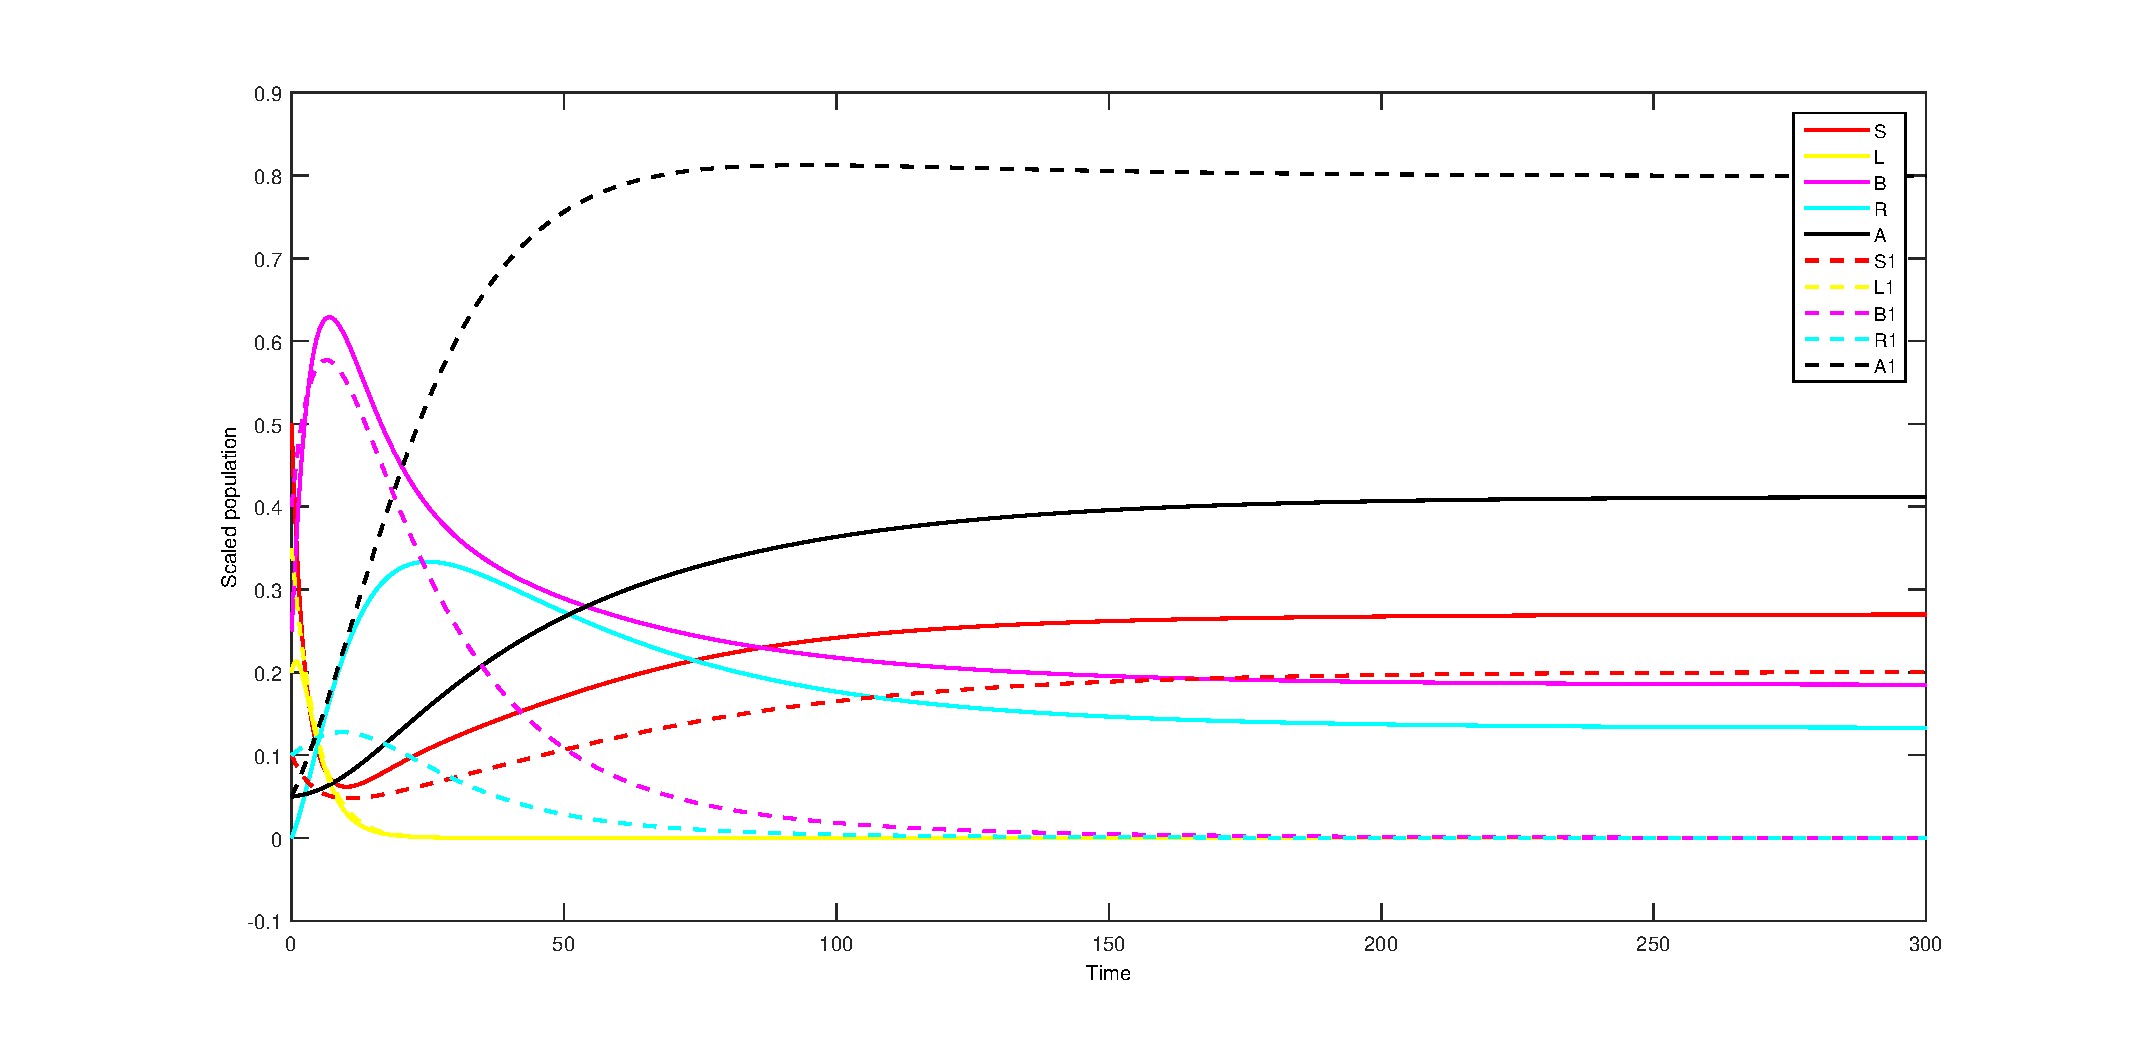
\includegraphics[width=3.5in,height=2.0in]{1.eps}\\
  \caption{Node Density vs. Time for different classes with Set 1}\label{fig:ff0}
\end{figure}

\indent Figure \ref{fig:ff0} is plotted with parameter Set 1 and initial points (0.5, 0.2, 0.25, 0, 0.05, 0.1, 0.35, 0.4, 0.1, 0.05). In this figure at steady state node density of $S$, $B$, $R$, $A$ and $S_{1}$ classes are greater than zero and possible feasible states are $E_{1}$, $E_{2}$, $E_{3}$, $E_{4}$, $E_{9}$ and $E_{10}$. Since all the reproduction number is greater than 1. Hence, we can conclude from the figure \ref{fig:ff0} that, $E_{9}$ is the stable steady state.\\
\begin{figure}
\centering
  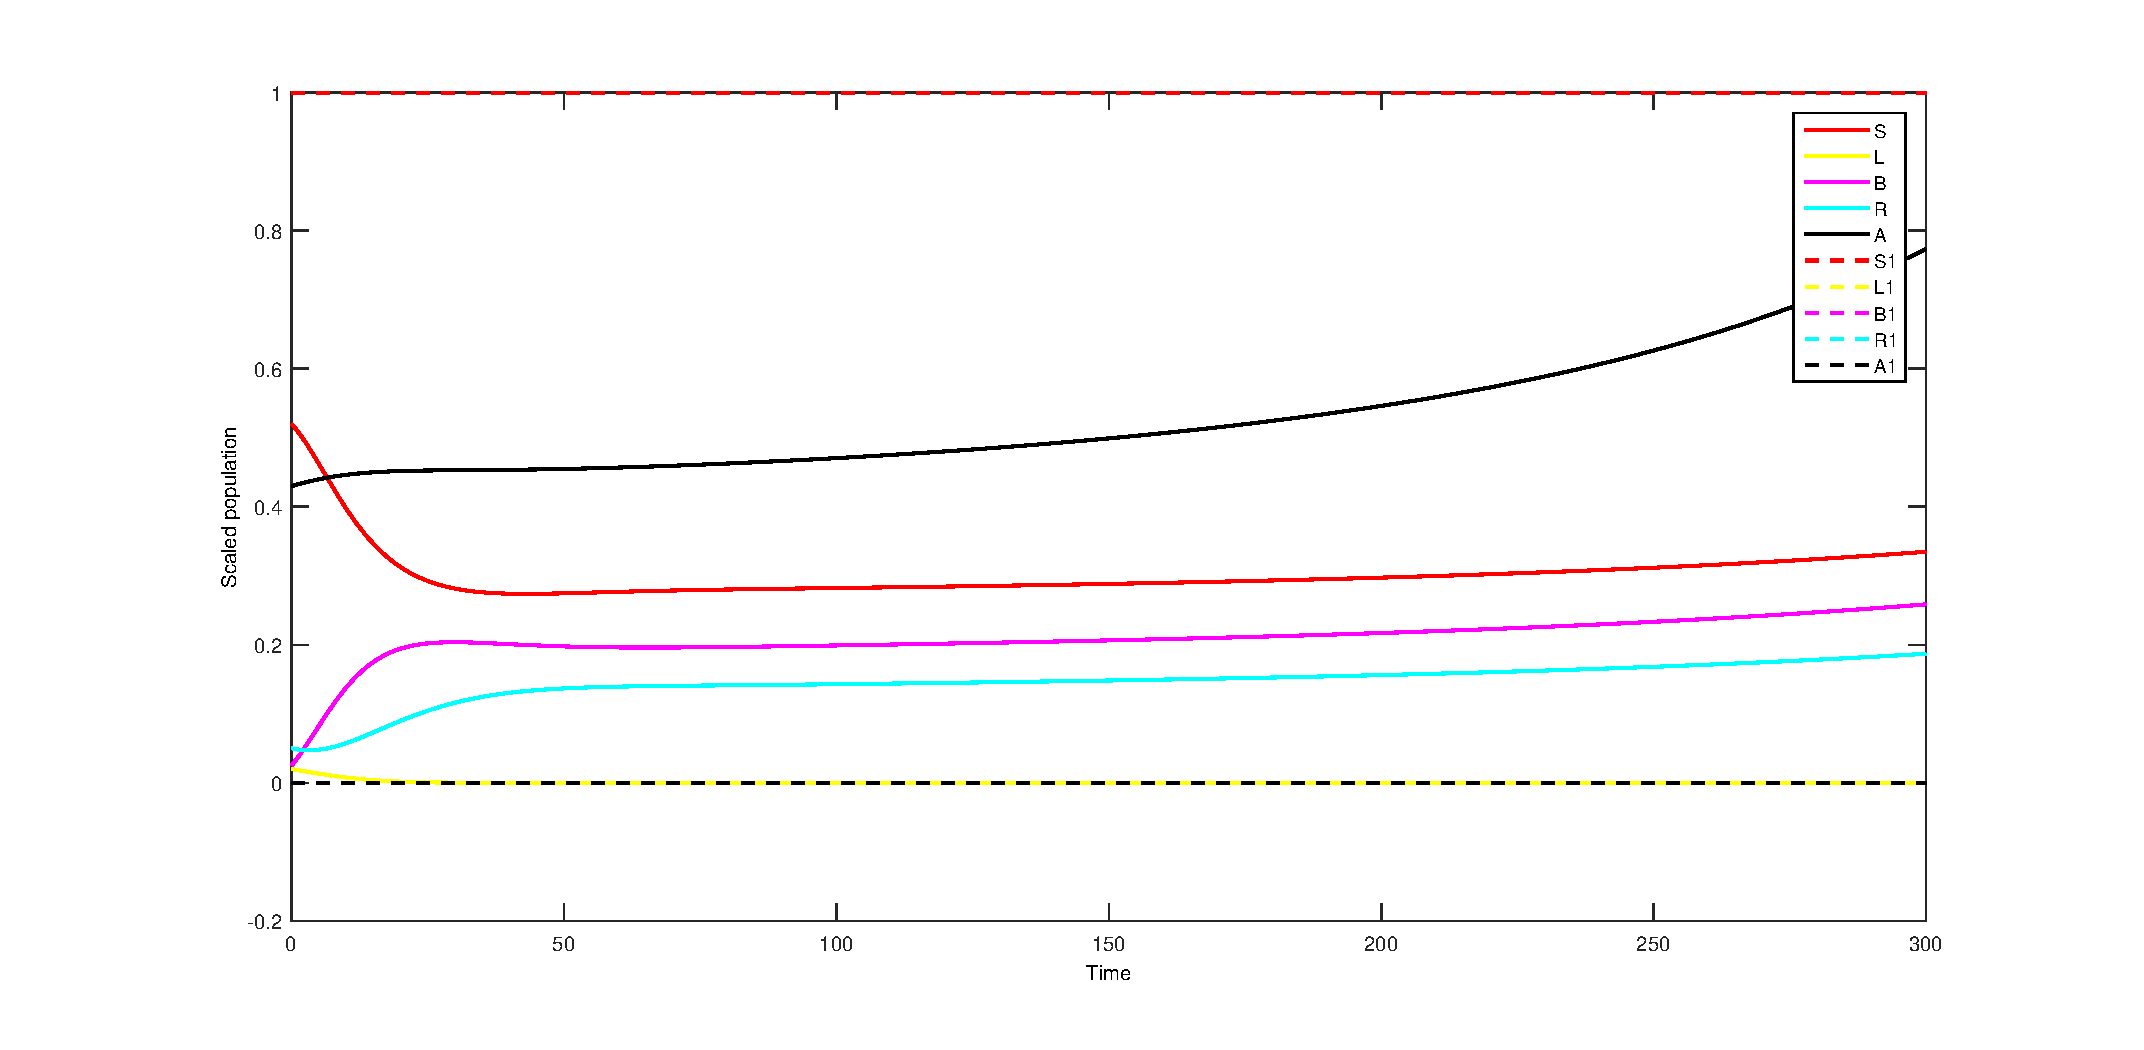
\includegraphics[width=3.5in,height=2.0in]{2.eps}\\
  \caption{Node Density vs. Time for different classes with Set 2}\label{fig:ff2}
\end{figure}
\indent Figure \ref{fig:ff2} is plotted with parameter Set 2 and initial points (0.5, 0.2, 0.25, 0, 0.05, 0.1, 0.35, 0.4, 0.1, and 0.05). Similarly, from the figure we can conclude that $E_{1}$, $E_{2}$, $E_{3}$ and  $E_{4}$ are the feasible steady states.

\begin{table}
\caption{Feasible steady states and numerical values of basic reproduction number for different parameter set in the model}\label{T1}
\centering
%\label{tab:equilibrium_SLBRA}
    \begin{tabular}{|p{1.9cm}|p{1.8cm}|p{1.8cm}|}
    \hline
               Parameters      & \textbf{Set 1} & \textbf{Set 2} \\
            \hline
  $\boldsymbol {\beta_{1}} $               & 0.6 & 0.6  \\
  $\boldsymbol {\beta_{2}} $                & 0.5 & 0.5  \\
  \textbf {k}      & 0.06 & 0.06 \\
  \textbf{c}               & 0.03 & 0.03 3\\
  $\boldsymbol{\alpha}$         & 0.05 & 0.05 \\
  $\mathbf {d _{2} }$          & 0.04 & 0.08 \\
  $\boldsymbol{\epsilon}$         & 0.3 & 0.3 \\
  $\boldsymbol{\gamma}$                & 0.045 & 0.45 \\
  $\boldsymbol{\delta}$       & 0.025 & 0.25\\
  \textbf{f}          & 0.02 & 0.02\\
  $\boldsymbol {\beta_{3}}$         & 0.4 & 0.4 \\
  $\boldsymbol {\beta_{4}}$            & 0.3 & 0.3\\
  $\mathbf{f_{1} } $        & 0.15 & 0.15\\
  $\mathbf{k_{1} }  $       & 0.05 & 0.05\\
  $\mathbf{c_{1} } $        & 0.01 & 0.01\\
  $\boldsymbol {\alpha_{1}}$         & 0.04 & 0.04 \\
  $\mathbf{d_{3}}$         & 0.05 & 0.05 \\
  $\boldsymbol {\gamma_{1}}$         & 0.035 & 0.35 \\
  $\boldsymbol {\delta_{1}}$        & 0.02 & 0.2 \\
  $\boldsymbol {\epsilon_{1}}$         & 0.25 & 0.25\\
  \hline
 \multirow{1}{4cm}{\small feasible SS}   &\scriptsize $E_{1},E_{2},E_{3},$ &\scriptsize $E_{1},E_{2},E_{3},E_{4}$ \\
  \hline
  ${{\cal R}}_{01}$ & 0.58803   & 0.9523  \\
  \hline
  ${{\cal R}}_{02}$ & 5.88034   & 0.9523  \\
  \hline
  ${{\cal R}}_{03}$ & 3.52822   & 0.8000 \\
  \hline
  ${{\cal R}}_{04}$ & 2.94421   & 0.4767  \\
  \hline
    \end{tabular}
\end{table}

\section{Estimation of firewall security coefficient}
The firewall is the core of a well-defined network security policy. The goal of the Check Point Firewall Rule Base is to create rules that only allow the specified connections.
\subsection{Order of Rule Enforcement}
The Firewall inspects connections and enforces the Rule Base in a sequential manner. The Firewall inspects each connection that comes to the network and compares the data (source, destination, service, etc.) to the first rule. If the connection matches the rule, the Firewall applies the action of that rule. If the connection does not match the rule, the Firewall continues with the next rule in the Rule Base.
\subsection{Firewall rule priority}
Because you can make firewall rules that have apparent conflicts, it is important to understand the order in which the rules are processed.
\subsection{Authenticated bypass}
These are rules in which the override block rules option is selected. These rules allow matching network traffic that would otherwise be blocked. The network traffic must be authenticated by using a separate connection security rule. You can use these rules to permit access to the computer to authorized network administrators and authorized network troubleshooting devices.
%\end{subsection}
\subsection{Block connection}
       These rules block all matching inbound network traffic.
%\end{subsection}
\subsection{Allow connection}
These rules allow matching inbound network traffic. Because the default  behavior is to block unsolicited inbound network traffic, you must create an allow rule to support any network program or service that must be able to accept inbound connections.

\indent The coefficient of firewall security, $m$ should depend on the types of files(data) under consideration, defined firewall security rules in the firewall rule base and the reliability and efficiency of the firewall. We propose a method for quantifying the coefficient m of firewall security as, $m=-{\log_e (p+q-pq)}$, where, $q$ quantifies the response of the files to the defined security rules.
For our work we can add certain rules by monitoring the behavior of attacker class. When the files will be received in targeted class, they will be checked according to the rules defined in the firewall rule base. If they response correctly to all these rules then $q=0$ and if they don't match any of the rules then $q=1$ and it is assumed that the malware propagation rate can be reduced by $p$ fraction, when all received files follow the defined security rules.

\begin{figure}
\centering
  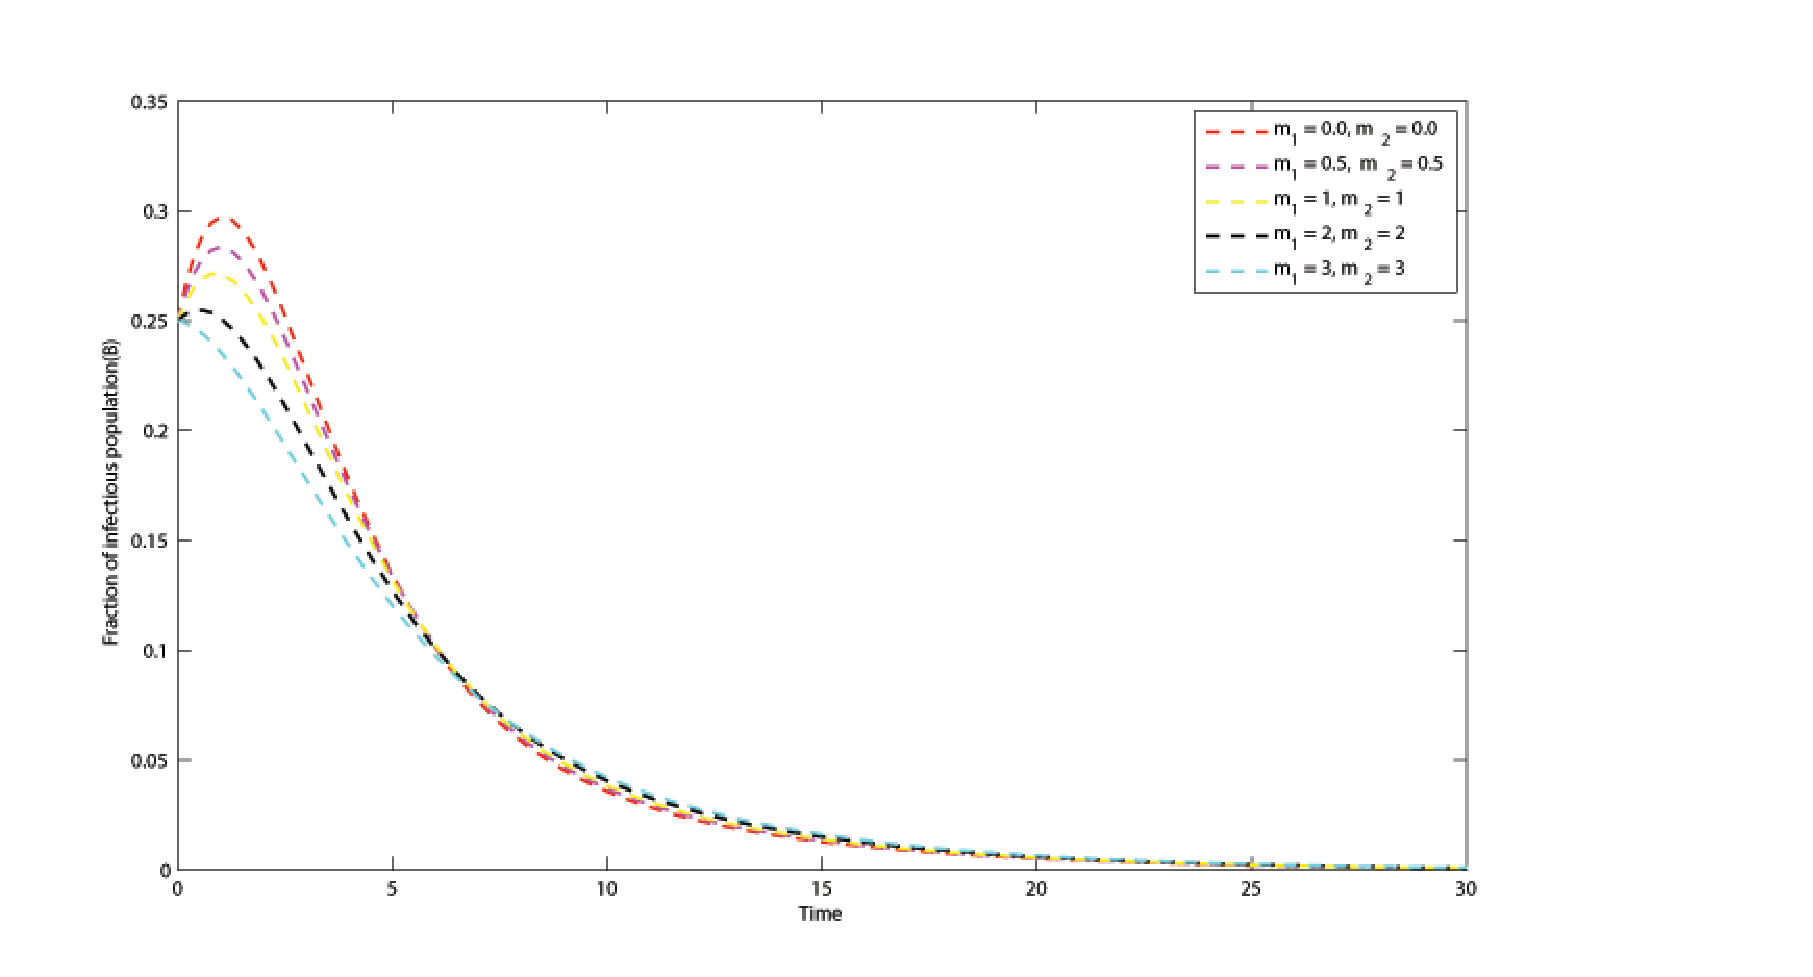
\includegraphics[width=3.5in,height=2.0in]{mB1.eps}\\
  \caption{Effect of $m$ on $B$ when $R_0<1$}\label{fig:ff3}
\end{figure}

\section{Conclusion}
In this work, an SLBRA epidemic model with distributed
attack on targeted resources is proposed and analyzed using stability theory of ordinary differential equations incorporating firewall security rule base. The important observations of this work are as follows:
\begin{itemize}
\item
For the proposed model sixteen equilibrium states are calculated out of which four are malicious codes free equilibrium and rest are endemic in nature. Basic reproduction number for
the disease free equilibrium states has been calculated and it has been found that if $R_{0} < 1$, then malicious code free equilibrium is stable and, if $R_{0} > 1$,
then the endemic equilibrium is stable. These conditions are verified by local
asymptotic stability of the system.

%\item
%An approach to estimate coefficient of firewall security $m$ is developed as
%
%          $$m=-{\log_e (p+q-pq)}$$
%
%where, $q$ quantifies the response of the files to the defined security rules. It is assumed that the malware propagation rate can be reduced by $p$ fraction when all received files follow the defined security rules.

\item
It is observed from the analysis that the coefficient of media coverage $m$ does not affect $R_{0}$ and hence the qualitative features of the model remains unaltered.

\item
We conclude that use of firewall security rule base helps to mitigate the problem of malicious code propagation in the network by lowering the level of infectious nodes at steady state.

\item
Finally, Normalized forward sensitivity indices are calculated for effective reproduction
number and state variables at endemic equilibrium with respect to various parameters and respective sensitive parameters are identified and shown in Table \ref{T2n}:

\begin{table}[ht!]
\caption{Sensitive Parameters}
\centering
\begin{tabular}{ |c|c| }
 \hline
  $R_{0}$ & Sensitive Parameters\\
  \hline
  $R_{01}$                  & $\beta_1,\beta_2,\beta_4$\\
  $R_{02}$                  & $\beta_1,\beta_2$  \\
  $R_{03}$                  & $\beta_2,\beta_3,\beta_4,k,c$ \\
  $R_{04}$                  & $\beta_1,\beta_2 ,k,c$\\
 \hline
\end{tabular} \label{T2n}
\end{table}
\end{itemize}


\section{Future Scope}
This work can be extended by adding more control strategies such as time delay for outbreak and time varying recruitment rate. Consider the following scenario, one day, Alice discovers that one of the programs she uses on her PC is infected with a virus. She eradicates it, in most models, this would be the end of the story. However, in this case Alice takes it upon herself to inform her friends Bob, Carol, and Dave, with whom she remembers having exchanged software sometime during the last few weeks. Simultaneously Bob, Carol and Dave eradicates virus if found and inform to their friends.This may be explained by a model in which, once a machine is found to be infected, neighboring machines are checked for viruses. This "kill signal" idea could be implemented in networks to greatly reduce the threat of viral spread\cite{kephart1993computers}. \\

\section*{Acknowledgment}
We are grateful to our Institution and colleagues whose constant encouragement served to renew spirit, refocus attention and energy and helped us in carrying out this work.

\addcontentsline{toc}{chapter}{REFERENCES}
\bibliographystyle{kluwer}
\bibliography{ref}

\end{document}


